\section{Transmission Media}\label{sec:transmission_media}
Different physical media carry the signals that transport our data across networks:

\subsection*{Guided Media}
Guided media confines signals to a specific path (literally "guided" along a cable or fiber). 

\subsubsection*{Twisted Pair Cable}
You probably know this one well, as you find it in most local area networks (LANs) and telephone systems. It consists of pairs of insulated copper wires twisted together to reduce electromagnetic interference.

\begin{figure}[h]
    \centering
    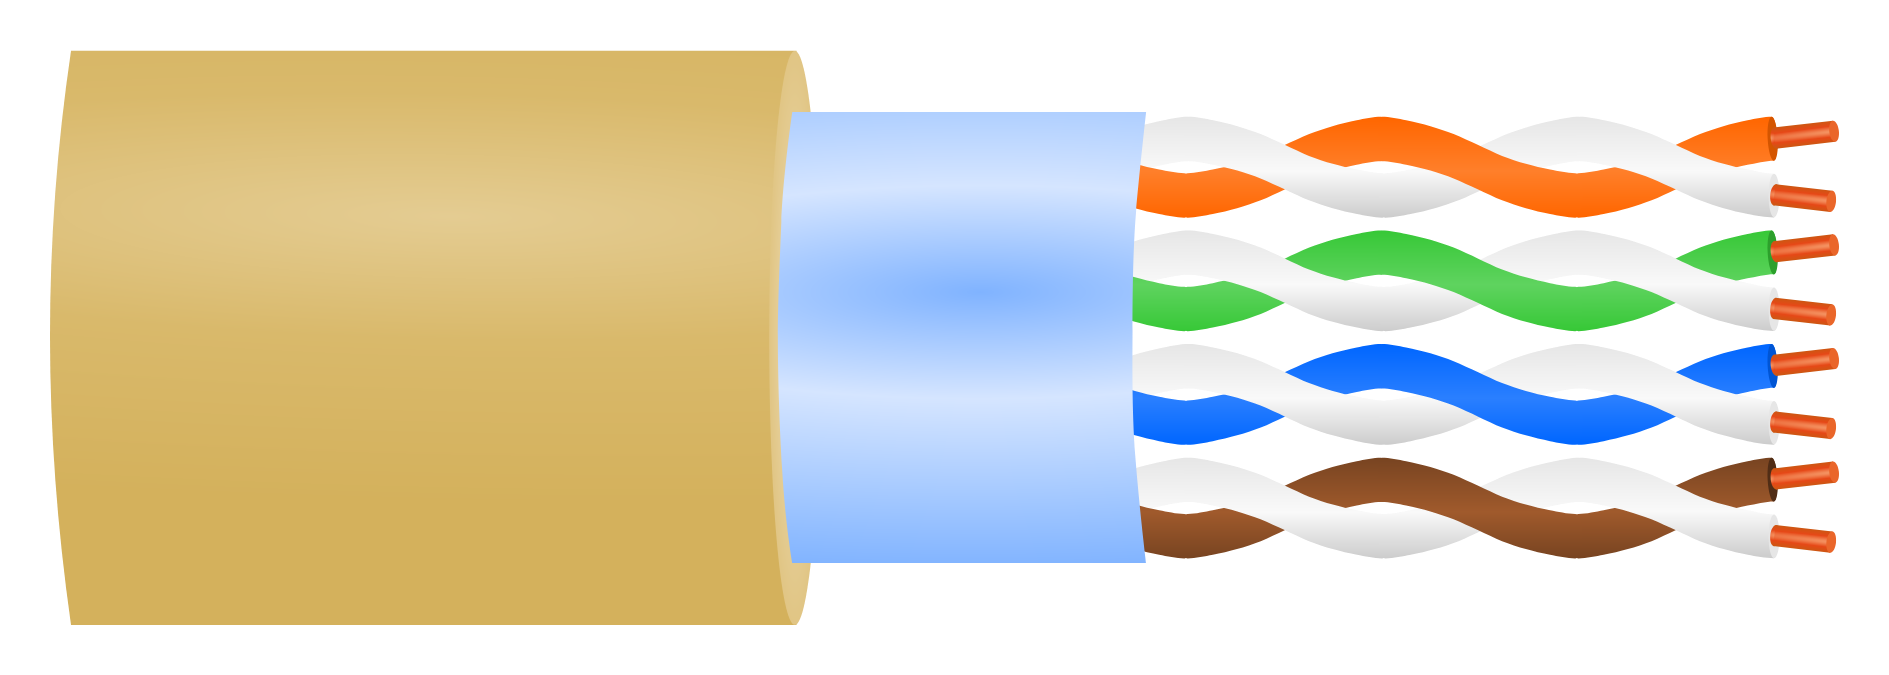
\includegraphics[width=4cm]{assets/osi/physical/f-utp.png}
    \caption{F-UTP}\label{fig:twisted_pair}
\end{figure}

UTP (Unshielded Twisted Pair) is the most common type, but there are also shielded variants like STP (Shielded Twisted Pair) and F/UTP (Foiled Unshielded Twisted Pair). There exist categories of TP cables abbreviated as \href{https://en.wikipedia.org/wiki/Category:Ethernet_cables}{Cat}, which you don't need to memorize, but should be aware of. 

\subsubsection*{Coaxial Cable}
Usually used in cable television and broadband\footnote{Everything but dial-up.}.

\begin{figure}[h]
    \centering
    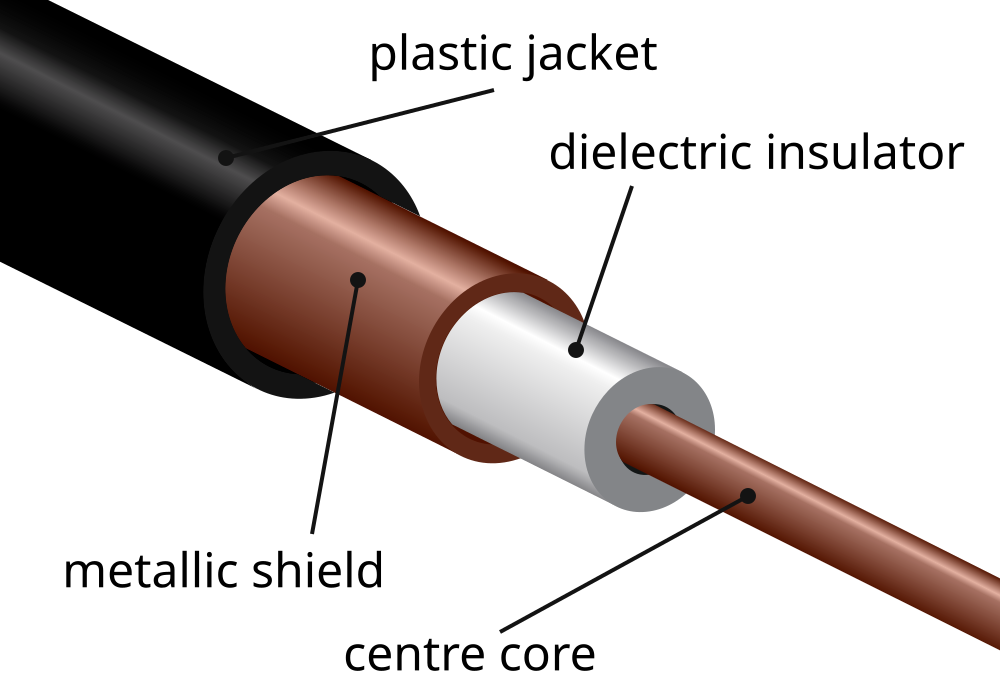
\includegraphics[width=4cm]{assets/osi/physical/coax.png}
    \caption{Coaxial cable structure}\label{fig:coaxial_cable}
\end{figure}

\begin{itemize}
    \item Common in cable TV networks and was used in early Ethernet implementations
    \item Offers better noise immunity than twisted pair with higher bandwidth capacity, which is why radio amateurs still use it
\end{itemize}

\vspace{1em}

\newpage
\subsubsection*{Fiber Optic Cable}
Uses light to transmit data, making it the fastest and most reliable medium available today.

\begin{itemize}
    \item Composed of a core, cladding, and protective outer layer
    \item Immune to electromagnetic interference
    \item Supports high bandwidths
\end{itemize}

\begin{figure}
    \centering
    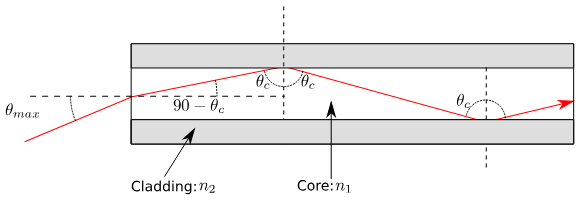
\includegraphics[width=.8\textwidth]{assets/osi/physical/fiber.png}
    \caption{Fiber optic cable structure}\label{fig:fiber_optic}
\end{figure}

\vspace{1em}

\subsection*{Wireless Transmission}
Ever wondered how signals travel through the air? Different types of electromagnetic waves are used for wireless communication, each with its own characteristics.

% assets/osi/physical/spectrum.png
\begin{figure}[h]
    \centering
    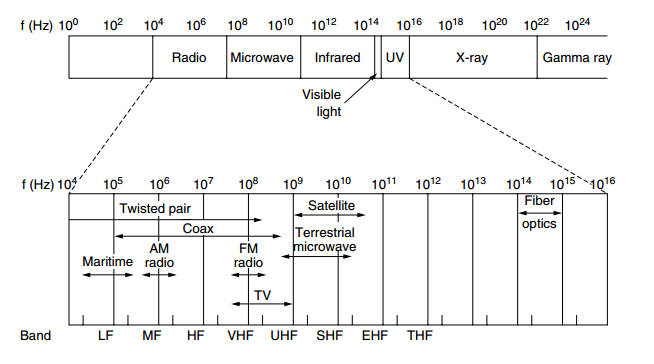
\includegraphics[width=.8\textwidth]{assets/osi/physical/spectrum.png}
    \caption{Electromagnetic spectrum showing different types of waves}\label{fig:em_spectrum}
\end{figure}

\subsubsection*{Radio Waves}
Radio waves are used for various wireless communication systems, including Wi-Fi, Bluetooth, and cellular networks. They can travel long distances (depending on wavelength) and penetrate through obstacles like walls.

\begin{noteblock}
    Fun fact! A lot of appliances like car remotes, thermostats and RC toys operate on the 433 MHz frequency band, which is a part of the radio spectrum. This is a perfect entry point if you'd like to hack your own devices or learn about radio communication.
\end{noteblock}

\subsubsection*{Microwaves}
Contrary to popular belief, microwaves are not just for cooking food. They are also used for point-to-point communication links, satellite communications, and some Wi-Fi networks. Microwaves have shorter wavelengths than radio waves, allowing them to carry more data, but faster attenuation\footnote{
    Attenuation: Reduction in signal strength as it travels through a medium, which can be caused by absorption, scattering, or reflection. 
    This is why we need repeaters/amplifiers!
} over distance.

\section{Standards and Specifications}
\subsection*{Ethernet Standards}
\begin{table}[h]
    \centering
    \begin{tabular}{|c|c|c|c|}
        \hline
        \textbf{Standard} & \textbf{Speed} & \textbf{Media} & \textbf{Distance} \\
        \hline
        10BASE-T & 10 Mbps & Cat3 UTP & 100m \\
        100BASE-TX & 100 Mbps & Cat5 UTP & 100m \\
        1000BASE-T & 1 Gbps & Cat5e UTP & 100m \\
        10GBASE-T & 10 Gbps & Cat6a UTP & 100m \\
        1000BASE-SX & 1 Gbps & Multi-mode fiber & 550m \\
        \hline
    \end{tabular}
    \caption{Common Ethernet Physical Layer Standards}\label{tab:ethernet_standards}
\end{table}

\begin{tipblock}
    The naming convention for Ethernet standards follows a pattern: \textbf{Speed + BASE + Medium}. For example, 100BASE-TX means 100 Mbps speed, baseband transmission, and twisted pair cable (T) with specific characteristics (X). The "BASE" indicates baseband\footnote{
        Baseband - entire medium is used for one signal at a time, as opposed to broadband where multiple signals can coexist. This is why Ethernet is often referred to as baseband transmission.
    } transmission (as opposed to broadband), and the suffix indicates the medium type: T for twisted pair, F for fiber, L for long-wavelength fiber.

    It's easier to remember if you think of it like this, instead of just memorizing the table.
\end{tipblock}


\subsection*{WiFi Standards}
\begin{itemize}
    \item 802.11a: 5 GHz, up to 54 Mbps
    \item 802.11b: 2.4 GHz, up to 11 Mbps
    \item 802.11g: 2.4 GHz, up to 54 Mbps
    \item 802.11n: 2.4/5 GHz, up to 600 Mbps
    \item 802.11ac: 5 GHz, up to 6.9 Gbps
    \item 802.11ax (WiFi 6): 2.4/5 GHz, up to 9.6 Gbps
\end{itemize}

\section{Signal Degradation}
Oh how we wish that signals could travel forever without losing strength! Unfortunately, they don't. As signals travel through a medium, they can degrade due to various factors like noise, interference, and attenuation.

This degradation can lead to errors in data transmission, which is why we need error detection and correction mechanisms in higher layers of the OSI model.

\subsection*{Shannon's Theorem and Channel Capacity}
Claude Shannon's groundbreaking work established the theoretical limits of data transmission over noisy channels. Shannon's theorem states that the maximum data rate (channel capacity) C of a noisy channel is given by:

\begin{equation}
C = B \log_2(1 + SNR)
\end{equation}

Where:
\begin{itemize}
    \item C = Channel capacity in bits per second (bps)
    \item B = Bandwidth in Hz
    \item SNR = Signal-to-Noise Ratio (linear, not in dB)
\end{itemize}

This formula tells us that even in the presence of noise, we can achieve error-free communication as long as our data rate doesn't exceed the channel capacity.

\subsection*{Nyquist's Theorem}
For noiseless channels, Harry Nyquist determined the maximum signaling rate. Nyquist's theorem states that the maximum data rate over a noiseless channel is:

\begin{equation}
C = 2B \log_2(V)
\end{equation}

Where:
\begin{itemize}
    \item C = Maximum data rate in bps
    \item B = Bandwidth in Hz
    \item V = Number of discrete signal levels
\end{itemize}

\begin{importantblock}
    Shannon's theorem considers noise and gives us the theoretical maximum for any channel, while Nyquist's theorem applies only to ideal, noiseless channels. In practice, Shannon's limit is more realistic since all real-world channels have noise.
\end{importantblock}

These theorems show us why we can't simply increase data rates indefinitely (which is something we really like doing when tackling complex problems) - physics imposes hard limits on information transmission!